%!TEX TS-program = xelatex
\documentclass{beamer}

\usepackage{HSE-theme/beamerthemeHSE} % Подгружаем тему

%%% Работа с русским языком и шрифтами
\usepackage[english,russian]{babel}   % загружает пакет многоязыковой вёрстки
\usepackage{fontspec}      % подготавливает загрузку шрифтов Open Type, True Type и др.

\defaultfontfeatures{Ligatures={TeX},Renderer=Basic}  % свойства шрифтов по умолчанию
% \setmainfont[Ligatures={TeX,Historic}]{KanjiStrokeOrders.ttf} %  установите шрифты Myriad Pro или (при невозможности) замените здесь на другой шрифт, который есть в системе — например, Arial
\setmainfont[ExternalLocation={./},Ligatures={TeX,Historic}]{MyriadPro-Regular.otf} %  установите шрифты Myriad Pro или (при невозможности) замените здесь на другой шрифт, который есть в системе — например, Arial
\setsansfont[ExternalLocation={./}]{MyriadPro-Regular.otf} %  установите шрифты Myriad Pro или (при невозможности) замените здесь на другой шрифт, который есть в системе — например, Arial
\setmonofont[ExternalLocation={./}]{MyriadPro-Regular.otf}
%\setmonofont{Courier New}

\uselanguage{russian}
\languagepath{russian}
\deftranslation[to=russian]{Theorem}{Теорема}
\deftranslation[to=russian]{Definition}{Определение}
\deftranslation[to=russian]{Definitions}{Определения}
\deftranslation[to=russian]{Corollary}{Следствие}
\deftranslation[to=russian]{Fact}{Факт}
\deftranslation[to=russian]{Example}{Пример}
\deftranslation[to=russian]{Examples}{Примеры}

\usepackage{multicol} 		% Несколько колонок
\graphicspath{{images/}}  	% Папка с картинками

\usepackage{color}
\usepackage{listings}

% remove caption prefix "Figure" from figures
\usepackage{caption}
\captionsetup[figure]{labelformat=empty}

% use this to excape underscores
\newcommand{\Code}[1]{\detokenize{#1}}

% use this to highlight in green for emphasis
\newcommand{\Green}[1]{\begin{exampleblock}#1\end{exampleblock}}

%%% Информация об авторе и выступлении
\title[Курсовая работа]{\scriptsize{%
Факультет компьютерных наук \\%
Департамент программной инженерии \\%
Курсовая работа \\%
}}

\subtitle{Программа скелетная анимация}

\author[Абрамов Артем 151 БПИ]{\scriptsize{%
Выполнил студент группы 151БПИ \\%
Абрамов Артем Михайлович \\%
Научный руководитель: \\%
доцент департамента программной \\%
инженерии, к.т.н \\%
Ахметсафина Римма Закиевна}}

%\institute[Высшая школа экономики]{Национальный исследовательский университет \\ «Высшая школа экономики» (Москва)}
\date{2016}

\begin{document}	% Начало презентации

\frame[plain]{\titlepage}	% Титульный слайд

%\section{Просто слайд с текстом}
%\subsection{Просто слайд с текстом}



%=============================================================
\begin{frame}
\frametitle{Предметная область}
\begin{multicols}{2}
\begin{small}
    Трехмерная компьютерная анимация - вид мультипликации, создаваемый при помощи компьютера. 
    \medskip
    
    В отличии от двухмерной анимаци, художник не рисует каждый кадр, а работает с моделью для которой последовательно задает различные позы.
\end{small}

\columnbreak
    
\begin{figure}[h!]
    \centering
    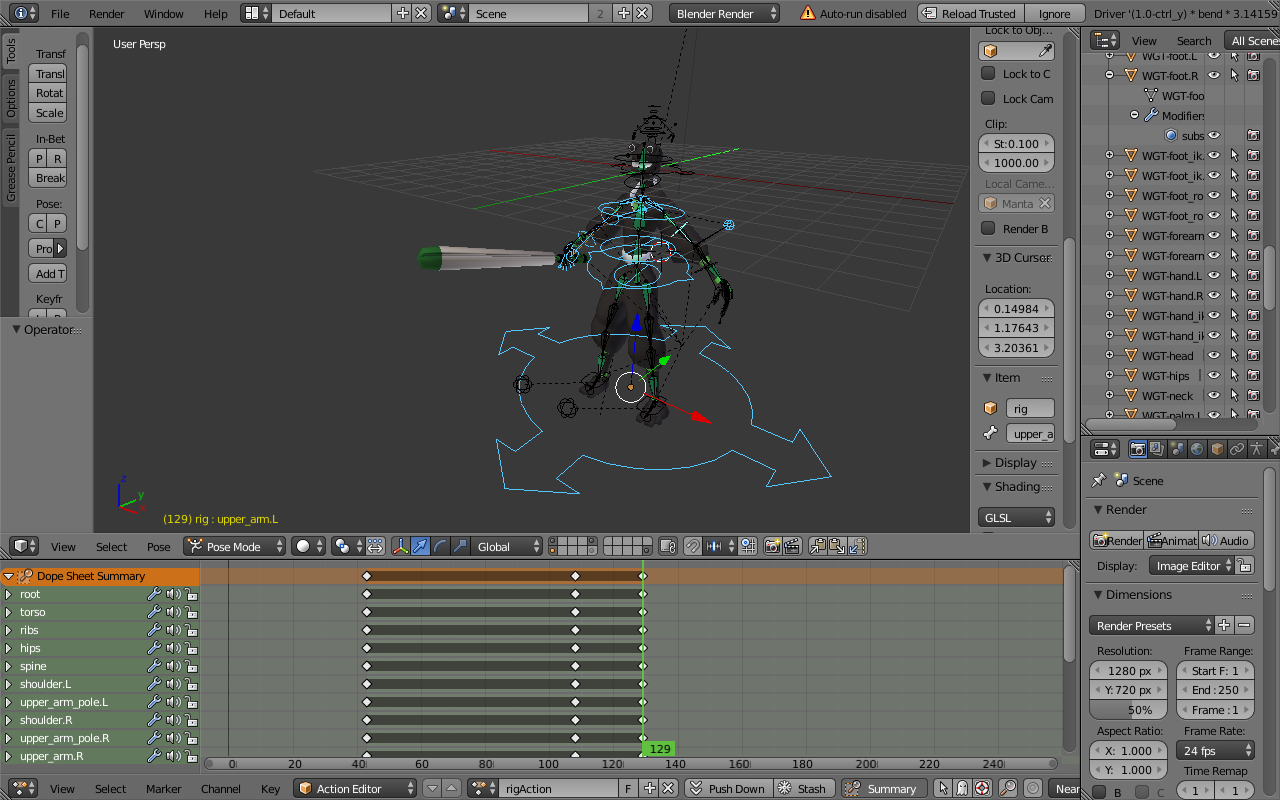
\includegraphics[width=1.15\columnwidth]{blender_at_work.png}
    \caption{Создание анимации в программе Blender}
    %\label{fig:awesome_image}
\end{figure}

\end{multicols}
\end{frame}


%=============================================================
\begin{frame}
\frametitle{Основные определения}

\begin{description}

\item[Корневая вершина дерева (англ. root node)]
Самый верхний узел дерева.

\item[Интерполяция, интерполирование анимации]
Способ нахождения промежуточных значений состояния анимации по имеющемуся дискретному набору известных значений.

\item[Матрица поворота (трансформации)]
Матрица 4х4, описывающая поворот, растяжение и сдвиг точек в трехмерном пространстве.

\item[OpenGL (Open Graphics Library)]
Спецификация, определяющая независимый от языка программирования платформонезависимый программный интерфейс для написания приложений, использующих двумерную и трёхмерную компьютерную графику. На платформе Windows конкурирует с Direct3D.

\end{description}
\end{frame}


%=============================================================
\begin{frame}
\frametitle{Обоснование актуальности работы}

\scriptsize{Отображение анимации - одна из наиболее актуальных задач  в производственной, научной и деловой сферах, а также в области развлечений.}
\begin{figure}[h!]
    \centering
    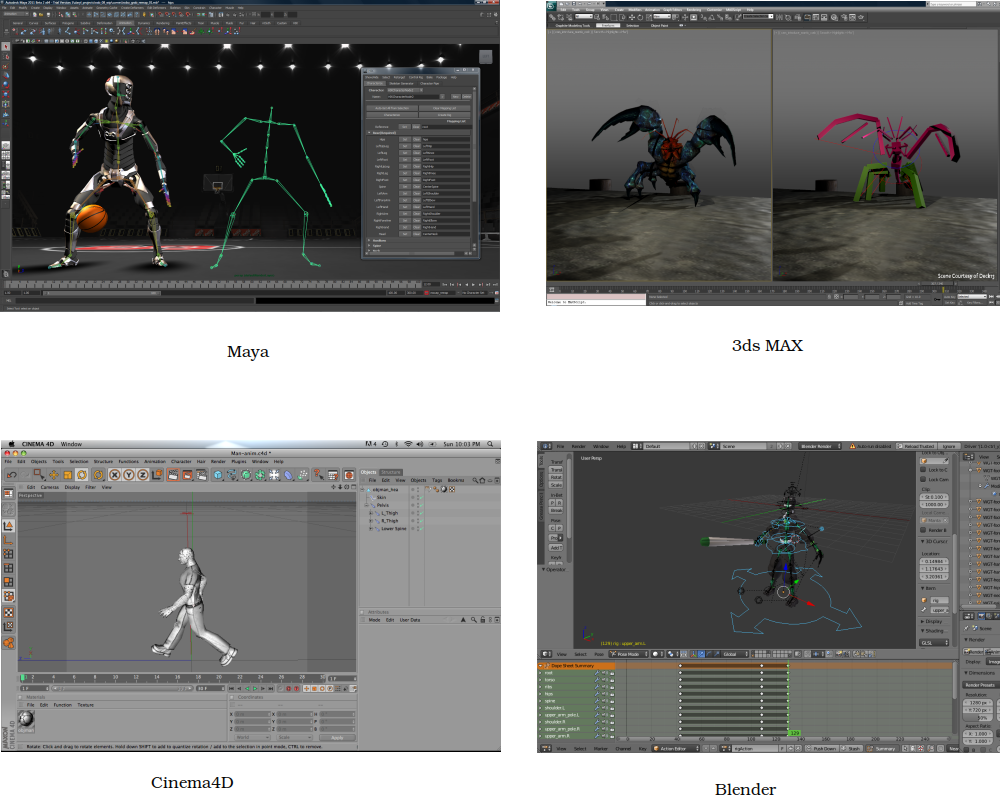
\includegraphics[width=0.7\textwidth]{all_tools.png}
    %\label{fig:awesome_image}
\end{figure}

\end{frame}



%=============================================================
\begin{frame}
\frametitle{Цели и задачи работы}
    Цель работы - реализовать программу скелетной анимации.
    
    \bigskip
    
    Задачи работы
    
    \smallskip
	\begin{enumerate}
	\item Рассмотреть различные подходы к анимации 3D моделей.
	\item Разработать структуры данных для хранения анимационных данных.
	\item Выбрать технологии для реализации.
	\item Изучить алгоритм скелетной анимации.
	\item Изучить технологию OpenGL.
	\item Реализовать программу.
	\item Разработать техническую документацию.
	\end{enumerate}
    
\end{frame}


%=============================================================
\begin{frame}
\frametitle{Различные подходы}
\begin{small}
    \alert{Неявные системы} используются, когда персонаж может совершать несколько действий одновременно и невозможно предугадать все возможные варианты анимации.
    
    \smallskip
    Предпочтение \alert{явным системам} отдается, когда необходимо анимировать большие группы людей или животных.
    
\begin{figure}[h!]
    \centering
    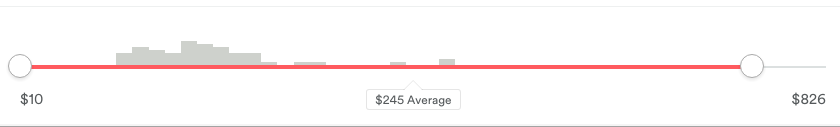
\includegraphics[width=1\textwidth]{raw_graph_cpu_vs_ram.png}
    %\caption{Шкала подходов к анимации, и отображающая позицию метода скелетной анимации}
    %\label{fig:awesome_image}
\end{figure}

\end{small}
\end{frame}



%=============================================================
\begin{frame}
\frametitle{Явные системы анимации}
\begin{scriptsize}
    Явная система - хранение отдельной модели для каждого кадра. \\
    После записи данных в файл, существует много методов для воспроизведения анимации.
    Такие методы требуют лишь элементарной математики. \\
    Однако типичная запись одного трэка анимации для одного персонажа занимает около 10MB (в формате MD3).
   
\begin{figure}[h!]
    \centering
    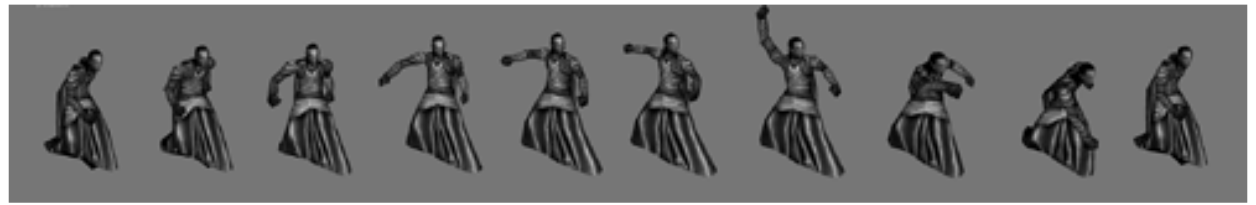
\includegraphics[width=1\textwidth]{explicit_animation.png}
    \caption{Каждому кадру соответствует своя модель}
\end{figure}

\end{scriptsize}
\end{frame}

  
%=============================================================
\begin{frame}
\frametitle{Неявные системы анимации}
\begin{scriptsize}
    Неявная система - хранение не моделей, а более высокоуровневого описания движения. \\
    В частности неявные \alert{системы скелетной анимации} содержат описание (через матрицу поворота) для каждой кости, как например локоть, плечо, шея. В реальном времени эти описания применяются к неанимированной модели для рассчета следующего кадра анимации. Эти рассчеты обычно требуют сложной математики с матрицами и тригонометрией. А следовательно и много CPU времени.
    
\begin{figure}[h!]
    \centering
    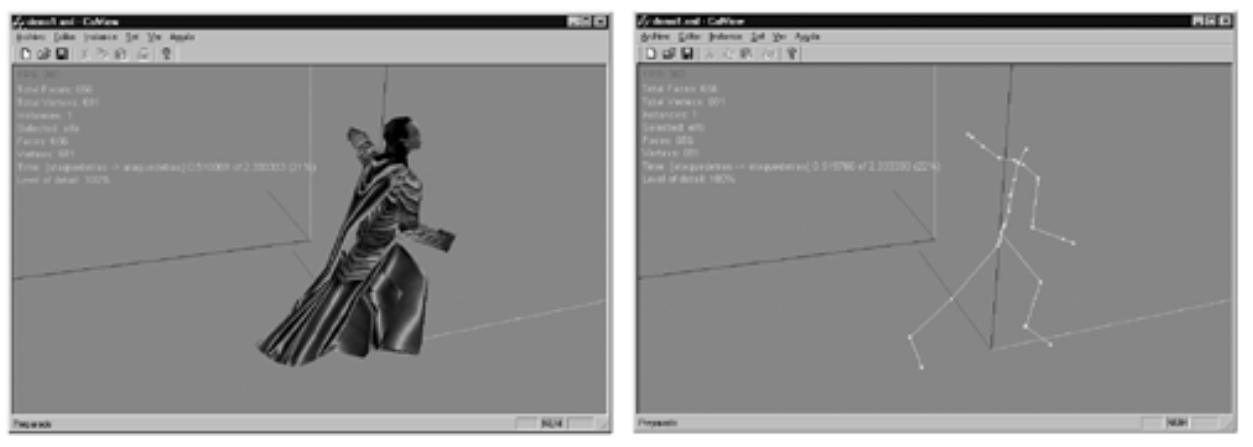
\includegraphics[width=0.8\textwidth]{implicit_animation.png}
    \caption{\scriptsize{Слева: анимированный персонаж; справа: скелет для данного кадра}}
    %\label{fig:awesome_image}
\end{figure}

\end{scriptsize}
\end{frame}


  
%=============================================================
\begin{frame}[fragile]
\frametitle{Структуры данных: Кость и Скелет}
\alert{Кость} содержит информацию о трех мерной трансформации (которая состоит из поворота, растяжения и смещения), а также информацию о кости-отце. Глобальная матрица для кости-потомка, - это произведение глобальной матрицы кости-родителя и матрицы кости-потомка. 

\medskip

\alert{Скелетом} называют иерархичную структуру сформированную костями. Скелет определяеться с помощью корневой кости в иерархии.

\begin{scriptsize}
\begin{figure}[h!]
\begin{verbatim}
class BoneNode
{
    public string Name;
    public Matrix4 GlobalTransform;
    public Matrix4 LocalTransform;

    public BoneNode Parent;
    public List<BoneNode> Children;
    public BoneNode(Node node_data) { ... }
}
\end{verbatim}
\end{figure}
\end{scriptsize}

\end{frame}


  
%=============================================================
\begin{frame}
\frametitle{Структуры данных: Трек анимации}
\begin{small}
В треке содержатся матрицы поворота скелета в ключевые моменты времени.
В упрощенном виде трек можно представить в качестве  массива пар: \\
$\lbrace$ время ключевого кадра, массив из матриц поворота для костей $\rbrace$

\begin{figure}[h!]
    \centering
    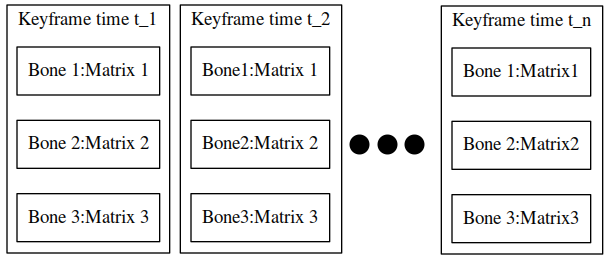
\includegraphics[width=0.6\textwidth]{anim_track.png}
    \caption{\scriptsize{В ключевые моменты времени \Code{(t_1, t_2, ... t_n)}, каждая кость ставится в соответствие с матрицей локальной трансформации.}}
\end{figure}


\end{small}
\end{frame}


  
%=============================================================
\begin{frame}[fragile]
\frametitle{Структуры данных: Модель}
\begin{scriptsize}

\begin{multicols}{2}
Модель состоит из набора вершин и весов вершин (коэффициент влиения кости на вершину). В пакете для трех мерной анимации каждая вершина модели «привязывается» к какой-либо кости скелета. Движение кости должно влиять на привязанные к ней вершины.

\columnbreak

\begin{verbatim}
struct Vbo
{
    public int QuantityIds;    
    public int VertexBufferId;
    public int NormalBufferId;
    public int ElementBufferId;
}
\end{verbatim}

\end{multicols}

\begin{figure}[h!]
    \centering
    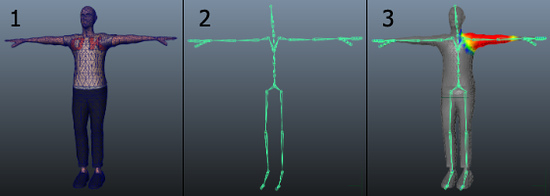
\includegraphics[width=0.6\textwidth]{skinning.png}
    \caption{\scriptsize{\textnumero 1 - модель; \textnumero 2 - скелет; \textnumero 3 - вершины модели, которые были привязанны к кости правого предплечья, выделенны красным}}
    %\label{fig:awesome_image}
\end{figure}

\end{scriptsize}
\end{frame}


%=============================================================
\begin{frame}
\frametitle{Алгоритм}
\begin{scriptsize}
В зависимости от времени из трека анимации извекаються данные о ключевом кадре.
Связь матриц с костями известна и можно применить извлеченные матрицы к скелету. 
Далее, так как известна связь костей с вершинами, можно применить трансформации костей к вершинам модели.

\begin{figure}[h!]
    \centering
    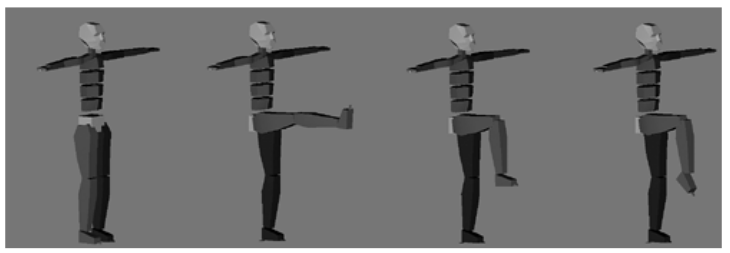
\includegraphics[width=1\textwidth]{forward_kinematics.png}
    \caption{\scriptsize{Применение преобразований, начиная от копчика (корневой кости) и заканчивая ступней.}}
    %\label{fig:awesome_image}
\end{figure}

\end{scriptsize}
\end{frame}


%=============================================================
\begin{frame}[fragile]
\frametitle{Применение трансформаций к скелету}
В треке матрицы поворота записаны относительно матрицы поворота родителя. 
Поэтому для анимации необходимо применять матрицы последовательно.
Начиная с корневой кости, примнить к ней описанную в треке анимации матрицу поворота.
Затем, двигаться вглубь скелета по иерархии и находить произведение матриц родителя и потомка (извлеченной из трека). В псевдокоде:
    
\begin{scriptsize}
\begin{lstlisting}
deform (bone, global matrix, track matrices)
  get matrix for bone from track matrices
  update global matrix
  store the result in bone as global transform
  if root has children
    deform (children of this node, global, track matrices)
  end if
end function
\end{lstlisting}
\end{scriptsize}

\end{frame}


%=============================================================
\begin{frame}[fragile]
\frametitle{Применение трансформаций к модели}
После того, как рассчитанны матрицы поворотов для скелета, их необходимо применить к вершинам модели.

\begin{scriptsize}
\begin{lstlisting}
deform (bone root, mesh original, mesh deformed)
  for each child_bone of root
    for each vertex in the original mesh
      if bone_weight > 0
          apply bone global transform to vertex
          scale the resulting point by the bone weight
          store the result in processeddata
      end if
    end for
    if child_bone has children
      deform (children of this node, mesh original, deformed)
    end if
  end for
\end{lstlisting}
\end{scriptsize}

\end{frame}




%=============================================================
\begin{frame}
\frametitle{Технологии и инструменты реализации}
\begin{itemize}
   \item Язык программирования C\#
   \item Библиотека \Code{Assimp v3.1 (http://assimp.org/)} для чтения файлов в формате collada (.dae).   
   \item Библиотека \Code{OpenTK v1.1.4 (http://www.opentk.com/)} для вызова функций OpenGL из C\# и предоставления базовых структур, например: Matrix4, Vector3.   
\end{itemize}
\end{frame}



%=============================================================
\begin{frame}[fragile]
\frametitle{Буферы памяти OpenGL}
	Загрузка данных о модели в OpenGL.
	Запрос OpenGL об отводе буферов памяти под вершины, нормали и массив индексов.
    
\begin{scriptsize}
\begin{lstlisting}
private void NewOpenGLBuf(out int bufId, List<Vector3D> data) 
{
    GL.GenBuffers(1, out bufId);
    GL.BindBuffer(BufferTarget.ArrayBuffer, bufId);    
    var byteCount = dataBuffer.Count * 12;
    var temp = new float[byteCount];
    foreach(var v in dataBuffer)
    {
       WriteIntoArray(temp, v);
    }
    GL.BufferData(BufferTarget.ArrayBuffer, (IntPtr)byteCount
            , temp, BufferUsageHint.StreamDraw);
}

private void Upload(out Vbo vboToFill)
{
    vboToFill = new Vbo();    
    NewOpenGLBuf(out vboToFill.VertexBufferId, _mesh.Vertices);
}
\end{lstlisting}
\end{scriptsize}
\end{frame}




%=============================================================
\begin{frame}[fragile]
\frametitle{Материалы в OpenGL}
	Загрузка данных о модели в OpenGL.
    Применение свойства материала, например: цвет, коэффициент рассеивания света, коэффициент свечения и т.д.
    
\begin{scriptsize}
\begin{lstlisting}
private void UseMaterial()
{
  color = Color2OpenTK(_material.ColorDiffuse);  
  GL.Material(MaterialFace.FrontAndBack, Material.Diffuse, color);  
  color = Color2OpenTK(_material.ColorAmbient);
  GL.Material(MaterialFace.FrontAndBack, Material.Ambient, color);

  color = new Color4(0, 0, 0, 1.0f);
  if (_material.HasColorEmissive)
  {
      color = color2OpenTK(_material.ColorEmissive);              
  }
  GL.Material(MaterialFace.FrontAndBack, Material.Emission, color);
}
\end{lstlisting}
\end{scriptsize}
  
\end{frame}





%=============================================================
\begin{frame}
\frametitle{Результаты работы}
    \begin{center}            
    \begin{large}
    Демонстрация
    \end{large}
    \end{center}
\end{frame}



%=============================================================
\begin{frame}
\frametitle{Выводы по работе}
    Пути дальнейшей работы:
\begin{enumerate} 
	\item Загрузка нескольких моделей
	\item Наложение матрицы трансформации на отдельные модели
	\item Выбор из нескольких трэков анимации
	\item Нанесение текстур
	\item Анимация на GPU
\end{enumerate}

\begin{figure}[h!]
    \flushright
    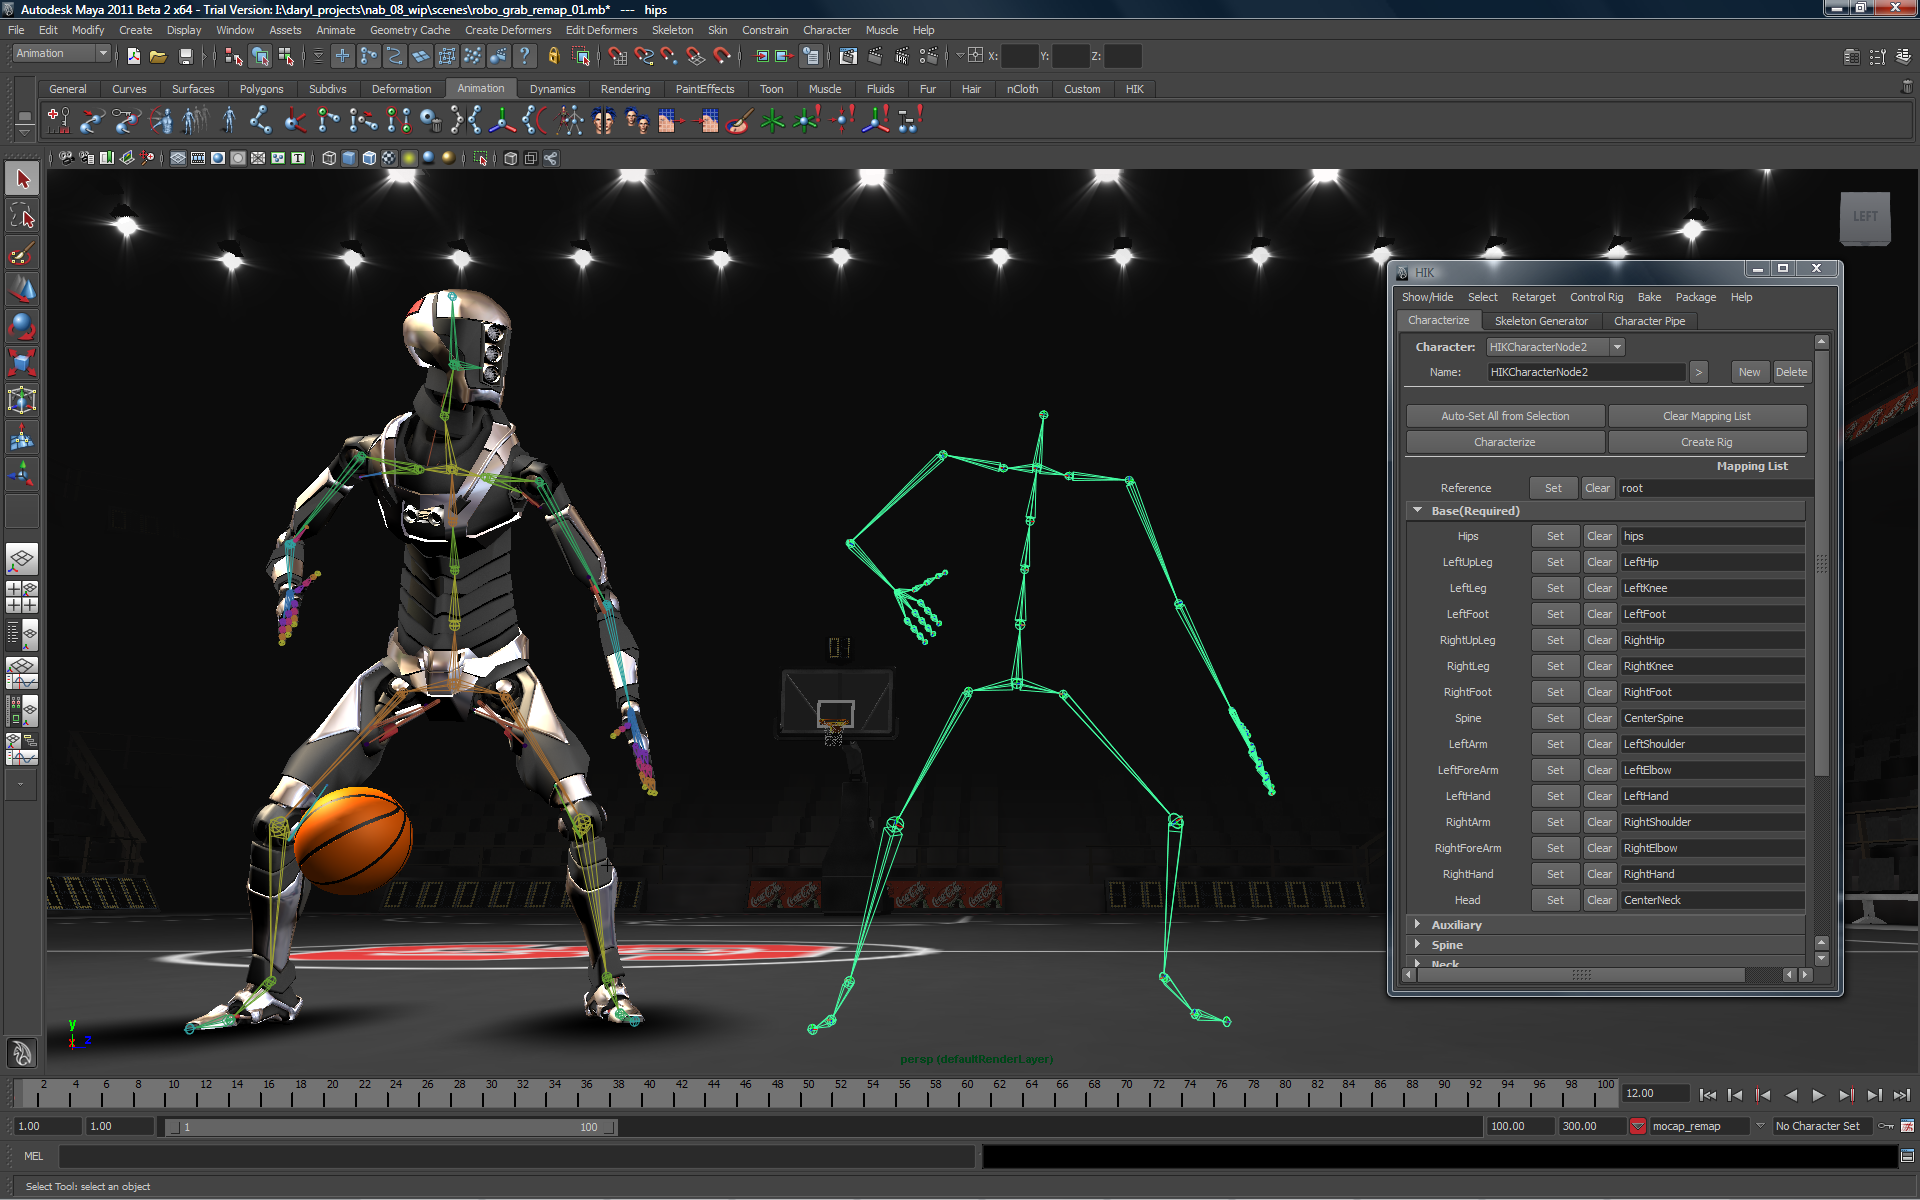
\includegraphics[width=0.6\textwidth]{win_maya.png}
    %\caption{\scriptsize{Схема логических блоков в программе}}
   %\label{fig:awesome_image}
\end{figure}

\end{frame}




%=============================================================
\begin{frame}
\frametitle{Список использованных источников}
\begin{itemize}
\item
Порев В.Н. Компьютерная графика. – СПб.: БХВ-Петербург, 2002. – 432 с.: ил.

\item 
Daniel S.D. Core Techniques and Algorithms in Game Programming/S.D. Daniel. - Springer, 2008 - 727 c.

\item
Документация OpenGL 3.3 [Электронный ресурс] // https://www.opengl.org/sdk/docs/man/ (Дата обращения: 21.10.2015, режим доступа: свободный)

\item
Рождерс Д. Алгоритмические основы машинной графики: Пер. с анг. - М.: Мир, 1989 - 512 с.
    
\end{itemize}
\end{frame}



\begin{frame}[c]
\begin{center}
\frametitle{\LARGE Спасибо за внимание!}

{\LARGE \inserttitle}

\bigskip

{\insertauthor}

\bigskip\bigskip

{\insertinstitute}

\bigskip\bigskip

{\large \insertdate}
\end{center}
\end{frame}

\end{document}
